\section{Prosjektil}

\subsection{Innledning}

Det fjerde og siste eksperimentet handlet om en prosjektilbevegelse. Dette er en bevegelse der et objekt skytes ut i luften, og kun påvirkes av akselerasjon gjennom tyngdekraften. Vi ser dermed bort fra luftmotstand i dette eksperimentet.

I en slik situasjon er bevegelsene på x- og y-aksen uavhengige, og vi kan regne med dem hver for seg. Det er dermed ingen akselerasjon i bevegelsen på x-aksen, mens y-aksen kun påvirkes av gravitasjonsakselerasjonen. Ved å vite dette kan vi ved hjelp av noen målinger finne ut mye om bevegelsen. Sentralt ligger bevaring av energi og de enkleste bevegelseslikningene.

Bevegelser som dette dukker opp ofte i fysikken. Vi vil ta for oss en prosjektilbevegelse i to dimensjoner, men en slik bevegelse kan beskrives i flere dimensjoner også

\subsection{Material og Metoder}

For eksperimentet trengte vi en prosjektilskyter (se fig \ref{projectile}), en prosjektil å skyte, en målestokk, 2 vanlige ark, et ark karbonpapir, og en mobiltelefon.

\bigskip \hfil
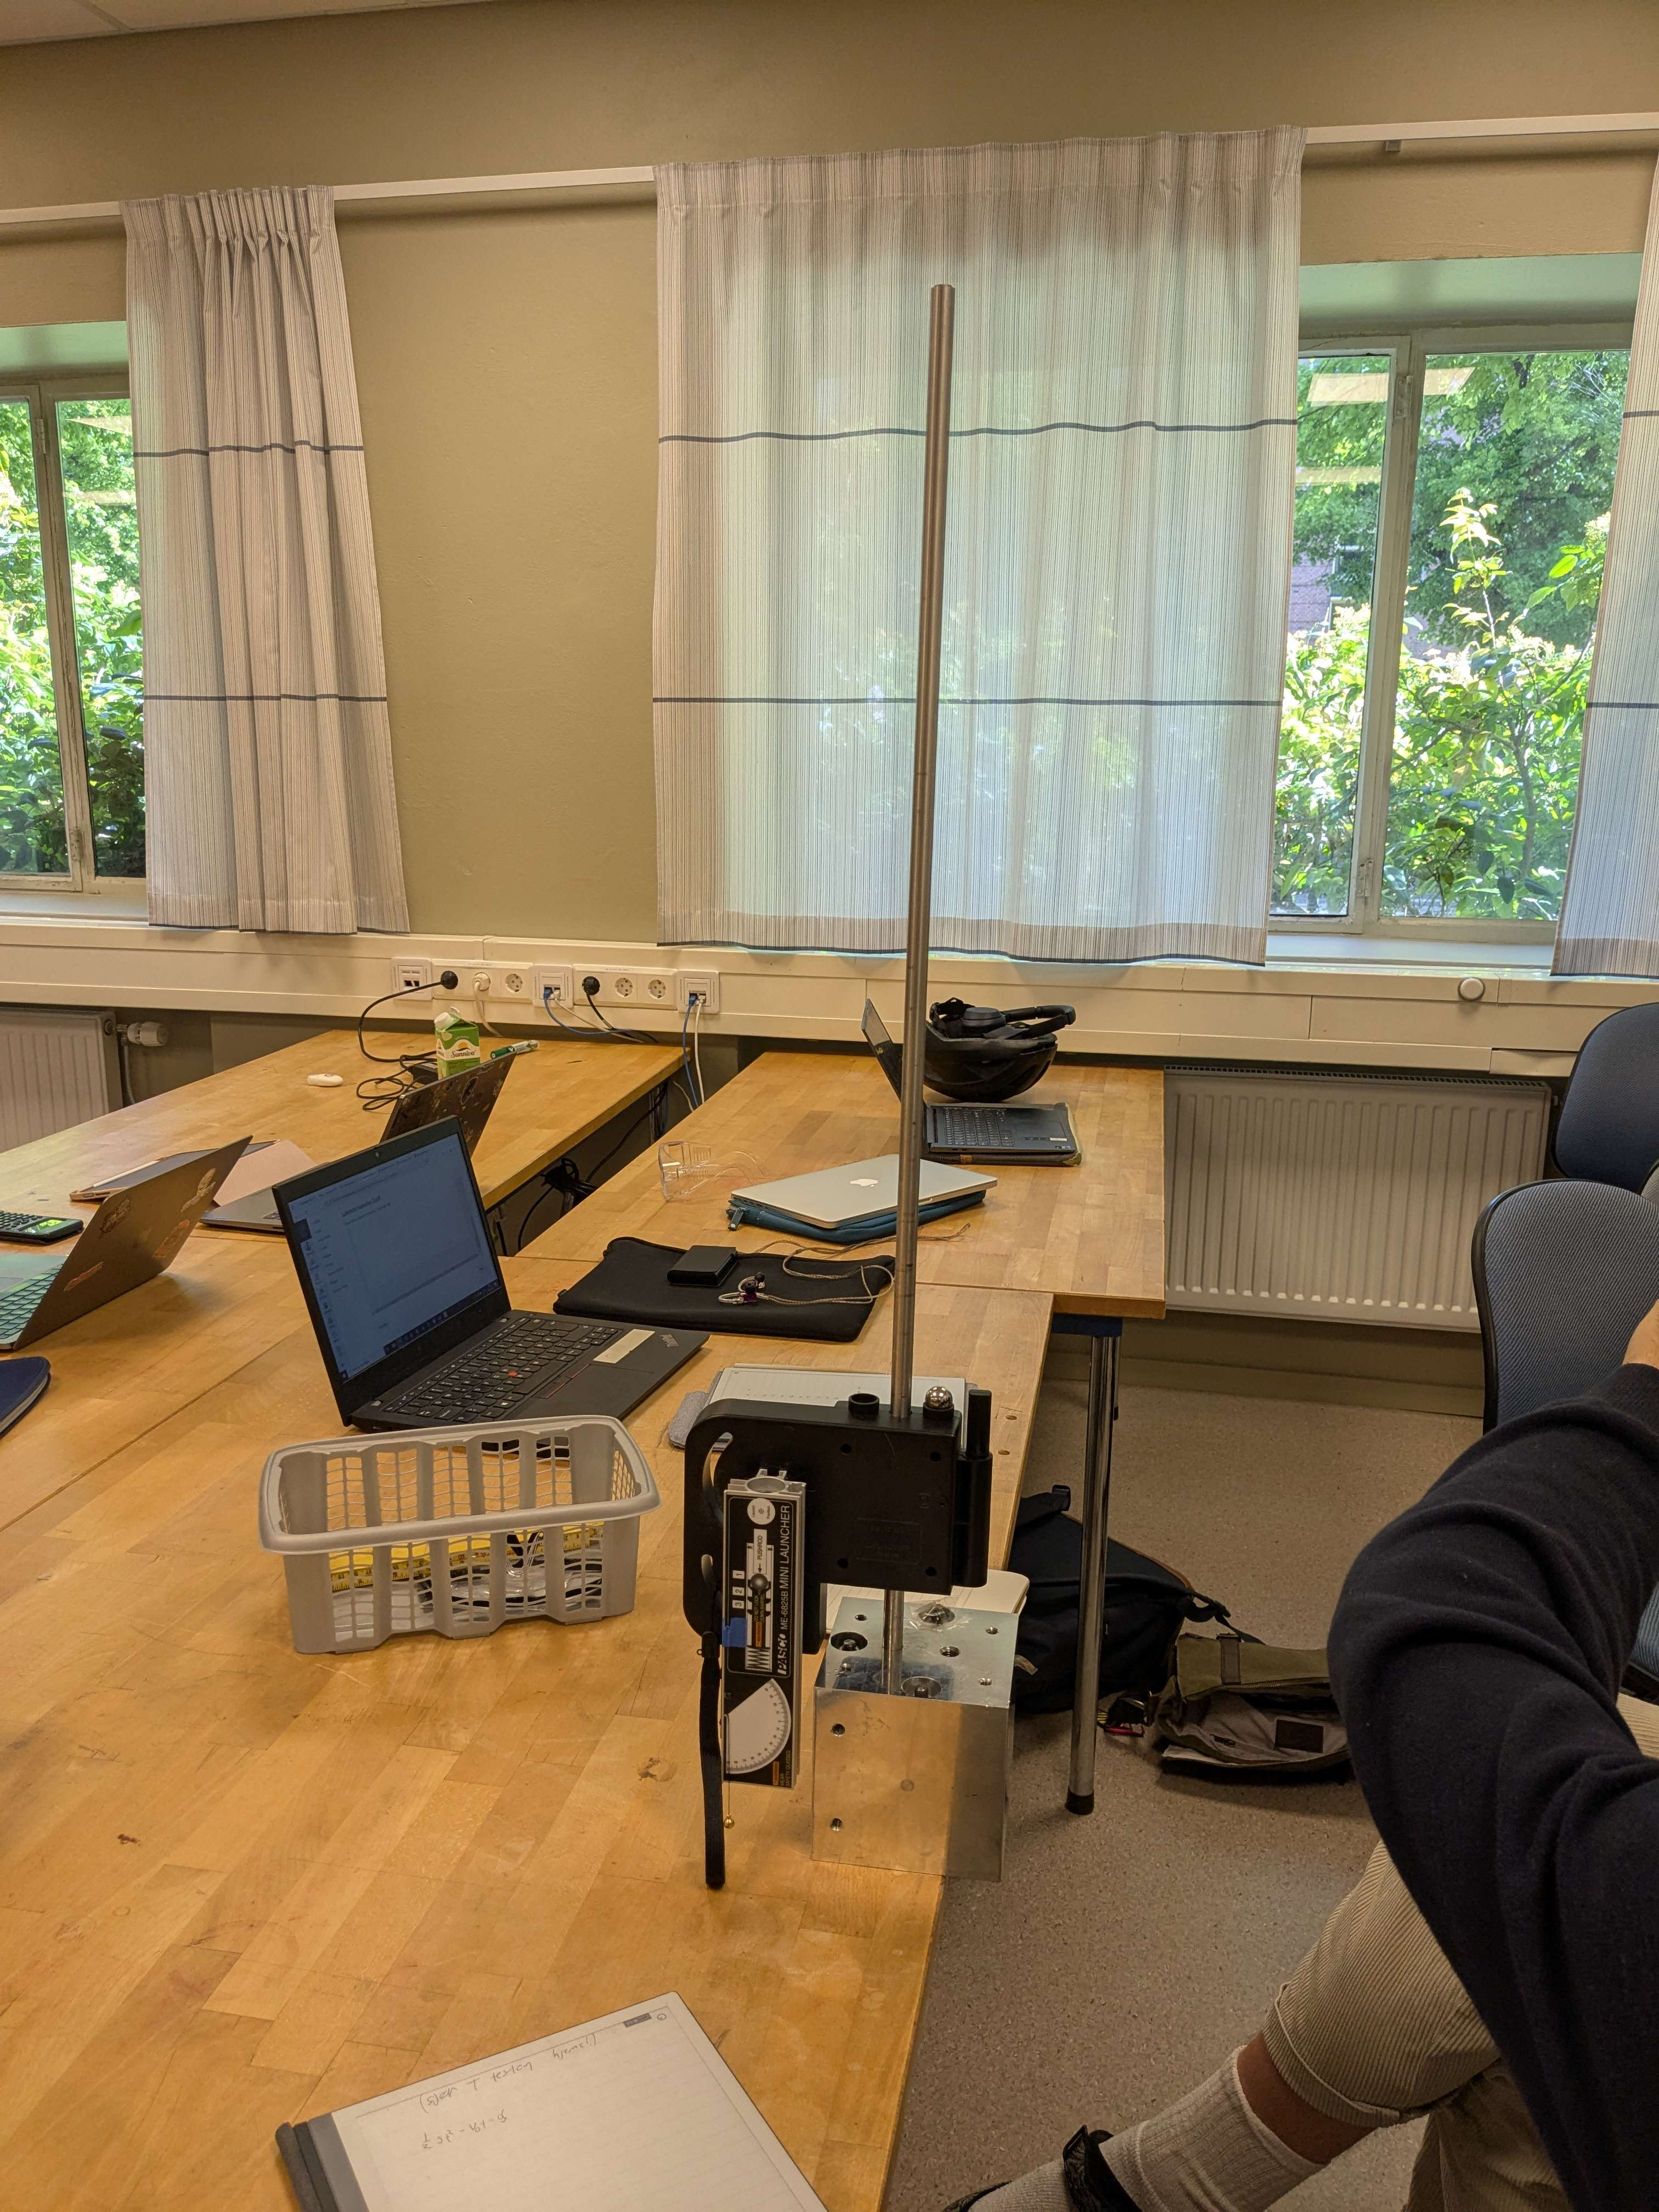
\includegraphics[scale = 0.05]{Figurer/Projectile.jpg} 
\captionof{figure}{Prosjektilskyteren}\label{projectile}
\par \bigskip

Først orienterte vi skyteren slik at prosjektilbevegelsen skulle bli et horisontalt kast, og så målte vi høyden fra bordet til prosjektilskyteren. Vi estimerte tiden dette kastet ville ta med følgende formel:

\begin{align}
    \hat{t} = \sqrt{\frac{2h_0}{g}}\label{that}
\end{align}

Så utførte vi en t-test for å sjekke om vi kunne måle tiden i et slikt kast. Vi brukte følgende formel for t-testen:

\begin{align}
    T = \left|\frac{t_{reaksjon} - \hat{t}}{u_{t_{reaksjon}}}\right|\label{ttest}
\end{align}

\medskip

Så orienterte vi skyteren slik at kastet ville bli kun vertikalt. Ved å måle det høyeste punktet prosjektilen når, kan vi bruke bevaring av energi

\begin{align}
    v_0 = \sqrt{2gh}\label{energy}
\end{align}

til å finne startfarten. Vi tok 20 mål av prosjektilens maksimale høyde. Vi gjorde dette ved å stille opp målestokken langs med prosjektilskyteren, skyte prosjektilen fra første hakk i skyteren, og filme området der prosjektilen var på sitt høyeste i slow-motion video, med mobiltelefonen. Slik kunne vi ganske nøyaktig plukke ut høyden. \medskip

Når vi hadde 20 mål for høyden, fant vi snittet av disse, og brukte det til å estimere starthastigheten. Vi brukte python for å gjøre dette. Programmet ga oss også et estimat for rekkevidden til et kast ved $\theta = 30^\circ$. Vi gjorde dette ved å først finne tiden (se formel \ref{timeformula}), og så hvor langt prosjektilen vil bevege seg på x-aksen (se formel \ref{xformula}):

\begin{align}
    t &= \frac{\sin{\theta}\cdot v_0 + \sqrt{(\sin{\theta})^2\cdot v_0^2 + 2gh_0}}{g} \label{timeformula}\\
\end{align}
\begin{align}
    x &= \cos{\theta}\cdot v_0 \cdot t \label{xformula}
\end{align}

Når vi hadde dette estimatet, orienterte vi skyteren slik at vi ville få et kast med $\theta = 30^\circ$. Så målte vi strektning lik rekkevidden vi hadde estimert, teipet vi et hvitt ark på bordet, og markerte estimatet vårt for rekkevidde på arket. Så plasserte vi karbonpapiret på toppen av det hvite arket, og så enda et hvitt ark på toppen av dette. Vi teipet så alle arkene ned til bordet. Så gjennomførte vi kastet med $\theta = 30^\circ$ 19 ganger, slik at prosjektilen landet på papirene. Når vi så tok av de to øverste arkene, hadde karbonpapiret markert hvor prosjektilen landet, slik at vi kunne måle hvor langt de hadde beveget seg.\medskip

Når vi målte strektningen for å plassere papiret, målte vi fra siden av skyteren, og ikke fra utskytningspunktet. Vi måtte dermed korrigere for det (se fig \ref{ProjDiagram})

\bigskip \hfil
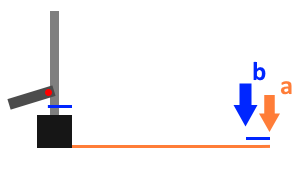
\includegraphics[scale = 0.5]{Figurer/ProsjektilDiagram.png} 
\captionof{figure}{a er strektningen vi målte til, som er litt for lang. b er den ordentlige strektningen fra utskytningspunktet, estimert i programmet.}\label{ProjDiagram}
\par \bigskip

Til slutt fant vi snittet av alle rekkeviddene vi målte, utførte en t-test for å sjekke om estimatet vårt var riktig, og plottet dataen. Formelen vi brukte for denne t-testen var:

\begin{align}
    T = \left|\frac{\overline{x} - \hat{x}}{SEM(x)}\right|\label{ttest2}
\end{align}

For å finne usikkerheten i en sum av andre usikre variabler, brukte vi følgende formel
\begin{align}
    u_f = \sqrt{u_x^2 +u_y^2}\label{au3}
\end{align}

Mer generelt anvendte vi 

\begin{align}
    u_f^2 = \left(\frac{\delta f}{\delta x} u_x\right)^2 + \left(\frac{\delta f}{\delta y} u_y\right)^2\label{gu2}
\end{align}

\subsection{Resultater}

Måle vårt for høyden på skyteren ble som følger:

\begin{center}
\begin{tabular}{ | c | c | }
    \hline
    $h_0$ & $u_{h_0}$ \\ 
    \hline
    21.4 & 0.0866\\ 
    \hline
\end{tabular}
\captionof{table}{Mål på utskytningspunktets høyde (i cm). Usikkerheten er funnet fra målestokkens skala- og ledd-usikkerhet, og en avlesningsusikkerhet. Alle disse var på 0.05cm, og $u_{h_0}$ ble funnet fra formel \ref{au3}}
\end{center}

Fra formel \ref{that} fikk vi $\hat{t} = 2.09$ s.  t-testen gir oss da $T = 8.2$, der grensen er $6.314$ for $T_{95}$ \medskip

Vi fikk 20 målinger for prosjektilens høyde i det vertikale kastet. Disse ligger i vedlegg \ref{Heights.txt}.

Programmet (vedlegg \ref{Get_h_line.py}) ga oss følgende estimater:

\begin{center}
\begin{tabular}{ | c | c | c | c | }
    \hline
    $\overline{h}$ (cm) & $v_0$ (m/s) & $\hat{t}$ (s) &  $\hat{x}$ (cm) \\ 
    \hline
    60.25 & 3.44 & 0.45 & 133 \\      
    \hline
\end{tabular}
\captionof{table}{Estimater fra programmet. Fra venstre til høyre: Snitthøyden i det vertikale kastet, startfarten estimert fra snitthøyden, den estimerte tiden i kastet med $\theta = 30^\circ$, og estimert distanse langs x-aksen i dette kastet.}
\end{center}

Mål på rekkeviddene i bevegelsen med $\theta = 30^\circ$ ligger vedlagt som vedlegg \ref{Lengths.txt}. Merk at avstandene er fra vårt estimat for rekkevidden, og ikke fra utskytningspunktet. Programmet lagt ved som vedlegg \ref{WorkWithLengths.py} ga oss følgende snittrekkevidde og usikkerhet:

\begin{center}
\begin{tabular}{ | c | c |  }
    \hline
    $\overline{x}$ & $SEM(x)$\\ 
    \hline
    $135.44$ & 0.093\\     
    \hline
\end{tabular}
\captionof{table}{Snittrekkevidde og usikkerhet i kast med $\theta = 30^\circ$, i cm.}
\end{center}

t-testen ga oss da T = 26.25, der grensen er 6.314 for $T_{95}$. \medskip

Programmet lagt ved som vedlegg \ref{WorkWithLengths.py} plottet også lengdene sammen med estimert rekkevidde:

\bigskip \hfil
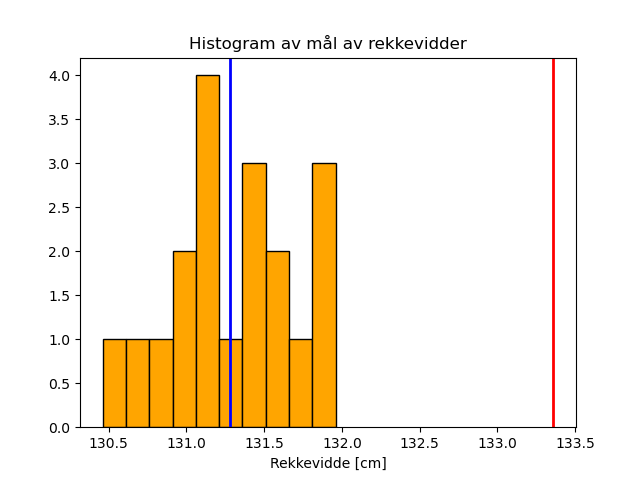
\includegraphics[scale = 0.75]{Figurer/HistRekkevidde.png} 
\captionof{figure}{Histogram av målte rekkevidder, sammen med estimert rekkevidde (rød) og snittrekkevidde (blå)}\label{RekkeviddeDiagram}
\par \bigskip


\subsection{Diskusjon}

Til og med før vi gjennomførte t-testen skjønte vi at vi ikke kunne måle tiden i det horisontale kastet, siden vi ikke ville reager i tide. t-testen bekreftet dette. Derfra valgte vi et vertikalt kast, slik at vi ikke må tenke på vinkler. 

Akkurat som i eksperiment 3 brukte vi slow-motion video til å finne høyden i det vertikale kastet. Dette kommer med begrensningen at mobiltelefonen har en grense på hvor mange bilder den kan ta i sekundet, men er fortsatt en mer nøyaktig måte å måle på enn øyemål.\medskip

For de målte rekkeviddene, kan vi se på histogrammet at estimatet er lenger vekk fra utskytningspunktet enn målene. Dette skyldes en systematisk feil sikkert :)

Noe om systematiske feil???